\section{Evaluation}
\label{discussion}

\subsection{Methodology}

The mobile application 'Are-U-Drunk?' has been tested with 8 people, aged from 18 to 58, 4 female and 8 male. The 8 participants were tested using the application once before drinking different amounts of alcohol and once after drinking it. If any inconvenience happpened (eyes could not be detected for any reason), the test was repeated. This mobile testing happened when and were the participant desired any time before drinking and 15-30 minutes after drinking. The day after the last mobile test, a form was provided to take a System Usability Scale (SUS) \cite{sus} test.

\subsection{Usability}

To test the usability of the system, SUS \cite{sus} has been used. This test is composed by 10 statements, in each of which the respondent states how they feel about the statement from 1 to 5, being 1 strongly disagree and 5 strongly agree. The 10 statements are the following.

\begin{itemize}
  \item I think that I would like to use this system frequently.
  \item I found the system unnecessarily complex.
  \item I thought the system was easy to use.
  \item I think that I would need the support of a technical person to be able to use this system.
  \item I found the various functions in this system were well integrated.
  \item I thought there was too much inconsistency in this system.
  \item I would imagine that most people would learn to use this system very quickly.
  \item I found the system very cumbersome to use.
  \item I felt very confident using the system.
  \item I needed to learn a lot of things before I could get going with this system.
\end{itemize}

\begin{figure}[h!]
  \centering
  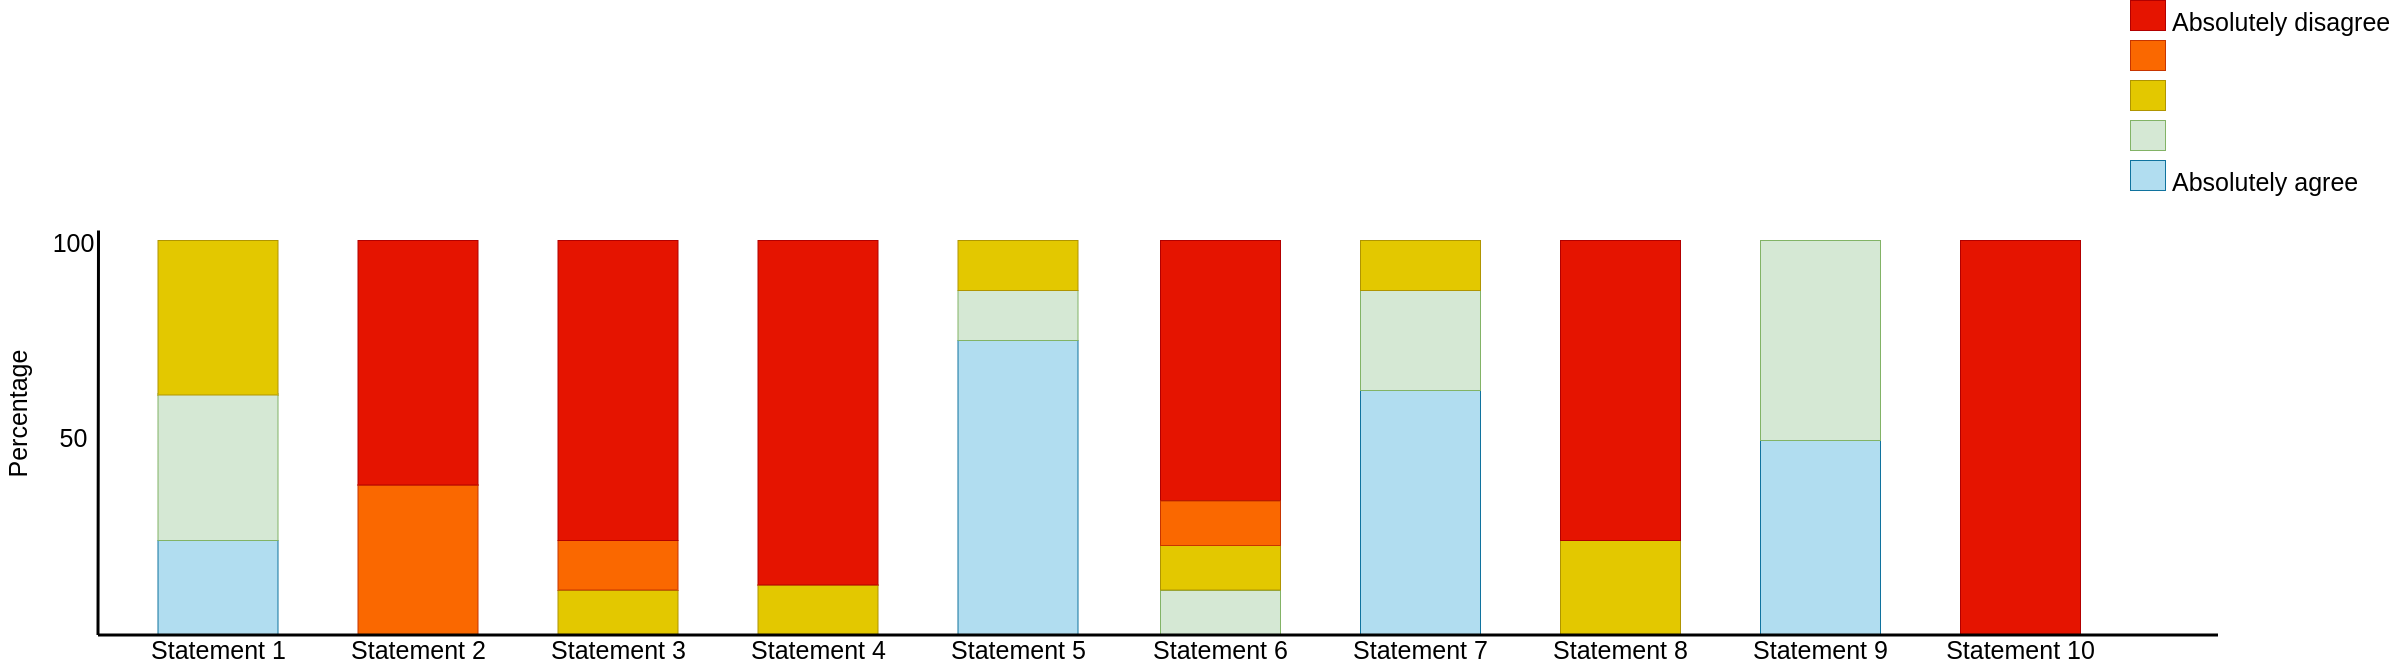
\includegraphics[angle=90, height=23cm,keepaspectratio]{./img/SUS.png}
  \caption{System Usability Scale responses' graph}
  \label{susgraph}
\end{figure}

Figure \ref{susgraph} represents the results. When asking if the participant would like to use this application frequently, 25\% strongly agreed, 37.5\% agreed and 37.5\% were neutral about the question. The system was not unnecessarily complex, 62.5\% of the users strongly disagreed about the application being complex and 37.5\% disagreed. 75\% of the participants strongly agreed the system was wasy to use, 12.5\% agreed and 12.5\% were neutral. Most of the participants, 87.5\%, strongly disagreed they would need the support of a technical person to be able to use the application and 12.5\% were neutral. When asking if the user found the various functions in the system were well integrated, 75\% strongly agreed, 12.5\% agreed and 12.5\% were neutral. The participants' opinions on whether there was too much inconsistency in this application are: 62.5\% strongly disagreed, 12.5\% disagreed, 12.5\% were neutral and 12.5\% agreed. 62.5\% of the users strongly agreed that most people would learn to use this system very quickly, 25\% agreed and 12.5\% were neutral. 75\% strongly disagreed the system was very cumbersome to use while 25\% was neutral about it. 50\% agreed they felt very confident using the application and 50\% strongly agreed. Finally, 100\% strongly disagreed they needed to learn a lot of thing before get going with the tests.

\subsection{Performance}



% Please add the following required packages to your document preamble:
% \usepackage{multirow}
\begin{table}[h!]
  % Please add the following required packages to your document preamble:
  % \usepackage{multirow}
  % Please add the following required packages to your document preamble:
  % \usepackage{multirow}
  % Please add the following required packages to your document preamble:
% \usepackage{multirow}
\begin{tabular}{|l|l|l|l|l|l|l|}
\hline
Participant                    & Gender                  & Age                 & Amount drank                                                                                  & Samples  & \begin{tabular}[c]{@{}l@{}}Before or \\ after \\ drinking\end{tabular} & Result     \\ \hline
\multirow{4}{*}{Participant 1} & \multirow{4}{*}{Female} & \multirow{4}{*}{25} & \multirow{4}{*}{Half a glass of wine}                                                         & Sample 1 & Before                                                                 & Null       \\ \cline{5-7}
                               &                         &                     &                                                                                               & Sample 2 & Before                                                                 & Fail       \\ \cline{5-7}
                               &                         &                     &                                                                                               & Sample 3 & After                                                                  & Undetected \\ \cline{5-7}
                               &                         &                     &                                                                                               & Sample 4 & After                                                                  & Fail       \\ \hline
\multirow{3}{*}{Participant 2} & \multirow{3}{*}{Male}   & \multirow{3}{*}{23} & \multirow{3}{*}{Half a glass of wine}                                                         & Sample 1 & Before                                                                 & Fail       \\ \cline{5-7}
                               &                         &                     &                                                                                               & Sample 2 & Before                                                                 & Fail       \\ \cline{5-7}
                               &                         &                     &                                                                                               & Sample 3 & After                                                                  & Fail       \\ \hline
\multirow{2}{*}{Participant 3} & \multirow{2}{*}{Male}   & \multirow{2}{*}{54} & \multirow{2}{*}{\begin{tabular}[c]{@{}l@{}}Two beers and \\ two glasses of wine\end{tabular}} & Sample 1 & Before                                                                 & Fail       \\ \cline{5-7}
                               &                         &                     &                                                                                               & Sample 2 & After                                                                  & Fail       \\ \hline
\multirow{3}{*}{Participant 4} & \multirow{3}{*}{Male}   & \multirow{3}{*}{18} & \multirow{3}{*}{Half a glass of wine}                                                         & Sample 1 & Before                                                                 & Fail       \\ \cline{5-7}
                               &                         &                     &                                                                                               & Sample 2 & After                                                                  & Undetected \\ \cline{5-7}
                               &                         &                     &                                                                                               & Sample 3 & After                                                                  & Fail       \\ \hline
\multirow{2}{*}{Participant 5} & \multirow{2}{*}{Female} & \multirow{2}{*}{53} & \multirow{2}{*}{A glass of wine}                                                              & Sample 1 & Before                                                                 & Fail       \\ \cline{5-7}
                               &                         &                     &                                                                                               & Sample 2 & After                                                                  & Fail       \\ \hline
\multirow{2}{*}{Participant 6} & \multirow{2}{*}{Male}   & \multirow{2}{*}{58} & \multirow{2}{*}{\begin{tabular}[c]{@{}l@{}}One and a half \\ rum and coke\end{tabular}}       & Sample 1 & Before                                                                 & Fail       \\ \cline{5-7}
                               &                         &                     &                                                                                               & Sample 2 & After                                                                  & Fail       \\ \hline
\multirow{2}{*}{Participant 7} & \multirow{2}{*}{Female} & \multirow{2}{*}{54} & \multirow{2}{*}{Half a rum and coke}                                                          & Sample 1 & Before                                                                 & Fail       \\ \cline{5-7}
                               &                         &                     &                                                                                               & Sample 2 & After                                                                  & Fail       \\ \hline
\multirow{3}{*}{Participant 8} & \multirow{3}{*}{Female} & \multirow{3}{*}{22} & \multirow{3}{*}{A beer}                                                                       & Sample 1 & Before                                                                 & Fail       \\ \cline{5-7}
                               &                         &                     &                                                                                               & Sample 2 & After                                                                  & Undetected \\ \cline{5-7}
                               &                         &                     &                                                                                               & Sample 3 & After                                                                  & Fail       \\ \hline
\end{tabular}
\caption{Subjects and samples of the application}
\label{subjects}
\end{table}

As Table \ref{subjects} shows, gender and age have been considered in the study participants, having an equal percentage of male and female people and a wide age range. Most of the tests are failed, three did not detect the eyes and one was quitted. The results of the tests were mainly 'fail'. Querying the database with the query shown in Listing \ref{dbquery}, we obtain the following data: 4 out of the 19 tests taken by all of the participants finished with only two clues, 6 finished with 3 clues, 5 finished with 4 clues and 6 finished in the 6th and last clue.

\begin{lstlisting}[caption={SQL query used to group the tests by the number of clues taken}, captionpos=b, label={dbquery}]
select acc, count(*) from (select count(*) as clues from public.clue group by father_test having count(*) > 1) as acc group by acc
\end{lstlisting}

The percentages of accuracy of eye movement in the failed clues were between 41.91\% and 56\% when the first two clues are failed. When the tests stopped at the third clue, the percentages varied from 50.86\% to 60\%, when the fourth was the last clue, the percentages were between 42.86\% and 60\% and finally, if the test finished with a failed last clue, the percentages varied from 50.36\% to 58.9\%. Some of the failed clues' videos were too dark, which may have caused the algorithm not to detect and track the eyes properly. Glasses also appear to affect the detection since all of the clues with a result of 'undetected' were taken with glasses. This may also affect the tracking of the eyes, but further research has to be done to affirm this. Furtuhermore, some of the videos were recorded too fast, meaning this that the eyes were moving faster than expected. After drinking, then number of passed clues was lower than the previous test when the participant was sober.
